% Set the document class and theme
\documentclass[notheorems]{beamer}

\setbeamertemplate{theorem}[ams style]
\setbeamertemplate{theorems}[numbered]

\makeatletter
    \ifbeamer@countsect
      \newtheorem{theorem}{\translate{Theorem}}[section]
    \else
      \newtheorem{theorem}{\translate{Theorem}}
    \fi
    \newtheorem{corollary}{\translate{Corollary}}
    \newtheorem{fact}{\translate{Fact}}
    \newtheorem{lemma}{\translate{Lemma}}
    \newtheorem{problem}{\translate{Problem}}
    \newtheorem{solution}{\translate{Solution}}

    \theoremstyle{definition}
    \newtheorem{definition}{\translate{Definition}}
    \newtheorem{definitions}{\translate{Definitions}}

    \theoremstyle{example}
    \newtheorem{example}{\translate{Example}}
    \newtheorem{examples}{\translate{Examples}}

    % Compatibility
    \newenvironment{Lemma}{\begin{lemma}}{\end{lemma}}
    \newenvironment{Proof}{\begin{proof}}{\end{proof}}
    \newenvironment{Theorem}{\begin{theorem}}{\end{theorem}}
    \newenvironment{Problem}{\begin{problem}}{\end{problem}}
    \newenvironment{Corollary}{\begin{corollary}}{\end{corollary}}
    \newenvironment{Example}{\begin{example}}{\end{example}}
    \newenvironment{Examples}{\begin{examples}}{\end{examples}}
    \newenvironment{Definition}{\begin{definition}}{\end{definition}}
\makeatother

\usetheme{Madrid}
\useoutertheme{miniframes} % Alternatively: miniframes, infolines, split
\useinnertheme{circles}

\definecolor{IITHorange}{RGB}{243, 130, 33} % UBC Blue (primary)
\definecolor{IITHyellow}{RGB}{254, 203, 10} % UBC Grey (secondary)

\setbeamercolor{palette primary}{bg=IITHorange,fg=white}
\setbeamercolor{palette secondary}{bg=IITHorange,fg=white}
\setbeamercolor{palette tertiary}{bg=IITHorange,fg=white}
\setbeamercolor{palette quaternary}{bg=IITHorange,fg=white}
\setbeamercolor{structure}{fg=IITHorange} % itemize, enumerate, etc
\setbeamercolor{section in toc}{fg=IITHorange} % TOC sections

% Override palette coloring with secondary
\setbeamercolor{subsection in head/foot}{bg=IITHyellow,fg=white}

\setbeamertemplate{caption}[numbered]
\setbeamertemplate{theorems}[numbered]

\usepackage{./presentation_macros}

\title{The Retracing Boomerang Attack}
\date{April 28, 2025}
\author{Gautam Singh}
\institute[IITH]{Indian Institute of Technology Hyderabad}

\begin{document}
    
    \begin{frame}
        \titlepage
    \end{frame}
    
    \begin{frame}
        \tableofcontents
    \end{frame}
    
    \section{Introduction}
    \label{sec:intro}
    
    \begin{frame}[<+->]{Introduction}
        \begin{enumerate}
            \item Broke the record for 5-round AES when it was
            published.
            \item Brings the attack complexity down to \(2^{16.5}\)
            encryptions.
            \item Uncovers a hidden relationship between boomerang attacks and
            two other cryptanalysis techniques: yoyo game and mixture
            differentials.
        \end{enumerate}
    \end{frame}

    \section{Preliminaries}
    \label{sec:prelims}

    \subsection{Boomerang Attacks}
    \label{subsec:boomerang}

    \begin{frame}{The Boomerang Attack}
        \begin{columns}
            \begin{column}{0.7\textwidth}
                \begin{enumerate}
                    \item<1-> Typically split the encryption function as 
                    \(E = E_1 \circ E_0\), with differential trails for each 
                    sub-cipher.
                    \item<2-> We can build a distinguisher that can distinguish
                    \(E\) from a truly random permutation in 
                    \(\cO\brak{\brak{pq}^{-2}}\) plaintext pairs.
                \end{enumerate}
            \end{column}
            \begin{column}{0.3\textwidth}
                \begin{figure}[!ht]
                    \centering
                    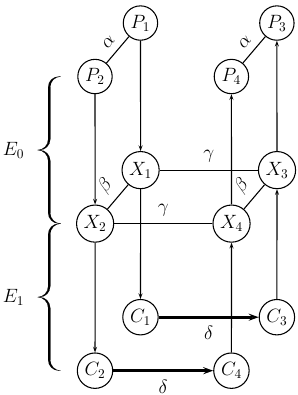
\includegraphics[width=\columnwidth]{images/boomerang.png}
                    \caption{The boomerang attack.}
                    \label{fig:boomerang}
                \end{figure}
            \end{column}
        \end{columns}
    \end{frame}

    \begin{frame}{The Boomerang Distinguisher}
        \vspace{-1em}
        \begin{algorithm}[H]
            \caption{The Boomerang Attack Distinguisher}
            \label{alg:boomerang-dist}
            \begin{algorithmic}[1]
                \State Initialize a counter \(ctr \gets 0\). 
                \State Generate \(\brak{pq}^{-2}\) plaintext pairs \(\brak{P_1, P_2}\)
                such that \(P_1 \oplus P_2 = \alpha\).
                \ForAll {pairs \(\brak{P_1, P_2}\)}
                    \State Ask for the encryption of \(\brak{P_1, P_2}\) to \(\brak{C_1,
                    C_2}\).
                    \State Compute \(C_3 = C_1 \oplus \delta\) and \(C_4 = C_2 \oplus 
                    \delta\). \Comment{\(\delta\)-shift}
                    \State Ask for the decryption of \(\brak{C_3, C_4}\) to \(\brak{P_3,
                    P_4}\).
                    \If {\(P_3 \oplus P_4 = \alpha\)}
                        \State Increment \(ctr\)
                    \EndIf
                \EndFor
                \If {\(ctr > 0\)}
                    \State \Return This is the cipher \(E\)
                \Else
                    \State \Return This is a random permutation
                \EndIf
            \end{algorithmic}
        \end{algorithm}
    \end{frame}

    \subsection{The S-box Switch}
    \label{subsec:s-box-switch}
    
    \begin{frame}[<+->]{Boomerang Switches}
        \begin{enumerate}
            \item Gain 1-2 middle rounds for free by choosing differentials 
            carefully. Here, we discuss the \emph{S-box switch}.
            \item Suppose the last operation in \(E_0\) is a layer of S-boxes 
            where \(S\brak{\rho_1\|\rho_2\|\ldots\|\rho_t} = 
            \brak{f_1\brak{\rho_1}\|f_2\brak{\rho_2}\|\ldots\|f_t\brak{\rho_t}}\)             
            for \(t\) independent keyed functions \(f_i\). Suppose the 
            difference for both \(\beta\) and \(\gamma\) corresponding to the 
            output of some \(f_j\) is equal to \(\Delta\). 
            \item Denoting this part of the intermediate state by \(X_j\),
            \begin{equation}
                \brak{X_1}_j \oplus \brak{X_2}_j = \brak{X_1}_j \oplus \brak{X_3}_j = \brak{X_2}_j \oplus \brak{X_4}_j = \Delta
                \label{eq:s-switch}
            \end{equation}
            which shows \(\brak{X_1}_j = \brak{X_4}_j\) and \(\brak{X_2}_j = 
            \brak{X_3}_j\).
            \item If the differential characteristic in \(f_j^{-1}\) holds for 
            \(\brak{X_1, X_2}\), then it will hold for \(\brak{X_3, X_4}\).
            \emph{We pay for probability in one direction}.
            \item Distinguisher probability increases by a factor of
            \(\brak{q^\prime}^{-1}\), where \(q^\prime\) is the probability of
            the differential characteristic in \(f_j\).
        \end{enumerate}
    \end{frame}

    \subsection{The Yoyo Game}
    \label{subsec:yoyo-game}
    
    \begin{frame}[<+->]{The Yoyo Game}
        \begin{enumerate}
            \item Similar to boomerang, starts by encrypting 
            \(\brak{P_1, P_2}\) to \(\brak{C_1, C_2}\), then modifying them to
            \(\brak{C_3, C_4}\) and decrypting them.
            \item \emph{Unlike} the boomerang attack, this process continues in
            the yoyo game.
            \item \emph{All} pairs of intermediate values 
            \(\brak{X_{2l + 1}, X_{2l + 2}}\) satisfy some property (such as 
            zero difference in some part).
            \item Probabilities are low with large \(l\). Still, the yoyo 
            technique has been used to attack AES reduced to 5 rounds.
        \end{enumerate}
    \end{frame}

    \subsection{Mixture Differentials}
    \label{subsec:mixture}
    
    \begin{frame}{Mixture}
        \begin{definition}[Mixture]
            \label{def:mixture}
            Suppose \(P_i \triangleq \brak{\rho_1^i, \rho_2^i, \ldots, 
            \rho_t^i}\). Given a plaintext pair \(\brak{P_1, P_2}\), we say 
            \(\brak{P_3, P_4}\) is a \emph{mixture counterpart} of 
            \(\brak{P_1, P_2}\) if for each \(1 \le j \le t\), the quartet 
            \(\brak{\rho_j^1, \rho_j^2, \rho_j^3, \rho_j^4}\) consists of two 
            pairs of equal values or of four equal values. The quartet 
            \(\brak{P_1, P_2, P_3, P_4}\) is called a \emph{mixture}.
        \end{definition}
        \pause
        \begin{enumerate}
            \item<2->  If \(\brak{P_1, P_2, P_3, P_4}\) is a mixture, 
            then XOR of the intermediate values \(\brak{X_1, X_2, X_3, X_4}\)
            is zero.
            \item<3-> \(X_1 \oplus X_3 = \gamma \implies X_2 \oplus X_4 = 
            \gamma\). Hence, for \(\gamma \xrightarrow{q} \delta\) in \(E_1\),
            \(C_1 \oplus C_3 = C_2 \oplus C_4 = \delta\) with probability
            \(q^2\).
            \item<4-> Has been applied to AES reduced up to 6 rounds. \(E_0\) 
            is taken to be the first 1.5 rounds of AES, which can be treated as
            four parallel super S-boxes.
        \end{enumerate}
    \end{frame}

    \section{The Retracing Boomerang Attack}
    \label{sec:retr-boomerang}
    
    \subsection{The Retracing Boomerang Framework}
    \label{sec:retr-framework}

    \begin{frame}{The Retracing Boomerang Framework}
        \begin{figure}[!ht]
            \centering
            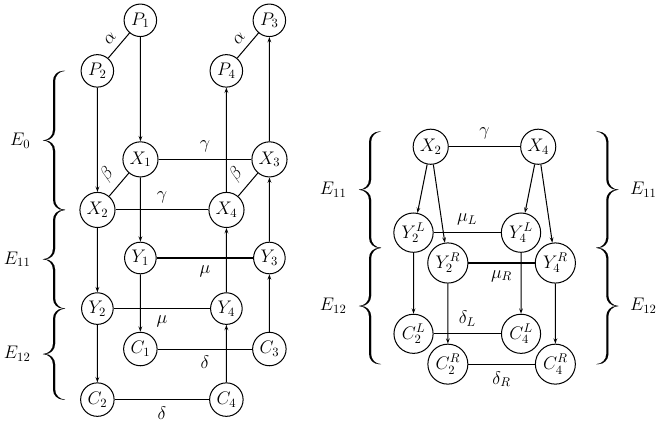
\includegraphics[width=0.6\columnwidth]{images/retracing_boomerang.png}
            \caption{The retracing boomerang attack.}
            \label{fig:retr-boomerang}
        \end{figure}
    \end{frame}

    \begin{frame}[<+->]{The Retracing Boomerang Attack}
        \begin{enumerate}
            \item The \emph{retracing boomerang} framework consists of a 
            \emph{shifting} type and a \emph{mixing} type.
            \item Both attacks use the setup shown in 
            \cref{fig:retr-boomerang}.
            \item Although the additional split looks restrictive, it applies 
            for a wide class of block ciphers such as SASAS constructions.
            \item Further, we assume that \(E_{12}\) can be split into two
            parts of size \(b\) and \(n - b\) bits, call these functions 
            \(E_{12}^L\) and \(E_{12}^R\), with characteristic probabilities
            \(q_2^L\) and \(q_2^R\) respectively.
        \end{enumerate}
    \end{frame}
\end{document}
